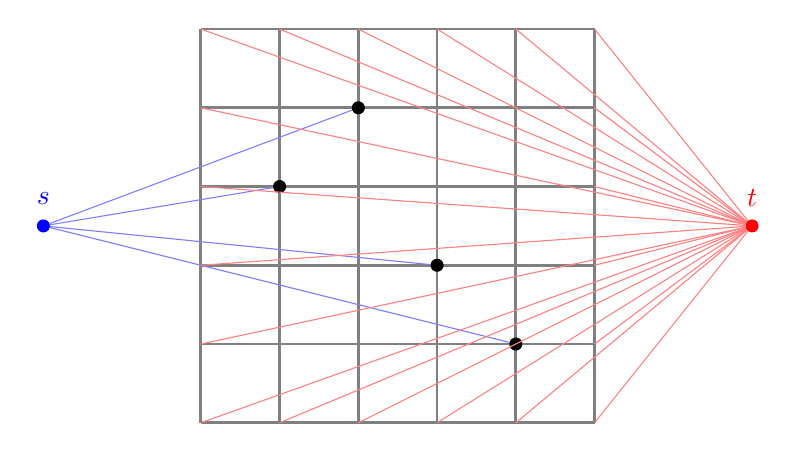
\begin{tikzpicture}[node distance=10pt]
\tikzstyle{blackdot} = [circle, fill, scale = 0.5];
\tikzstyle{starter} = [blue!50];
\draw[help lines,line width=1pt]  (-2,2) grid (3,-3);
\node [blackdot] (v3) at (0,1) {};
\node [blackdot] (v2) at (-1,0) {};
\node [blackdot] (v4) at (1,-1) {};
\node [blackdot] (v5) at (2,-2) {};

\node [blackdot,blue] (v1) at (-4,-0.5) {};
\draw [starter] (v1) edge (v2);
\draw [starter] (v3) edge (v1);
\draw [starter] (v4) edge (v1);
\draw [starter] (v5) edge (v1);

\node [blackdot,red] (t) at (5,-0.5) {};
\foreach \x in {-2,-1,...,3}
	\foreach \y in {2,-3}
		\draw[red!50] (\x,\y) edge (t);
\foreach \x in {-2,3}
	\foreach \y in {1,0,...,-2}
		\draw[red!50] (\x,\y) edge (t);

\node [above of=v1,blue] {$s$};
\node [above of=t,red] {$t$};
\end{tikzpicture}